%********************************************************************
% Appendix
%*******************************************************
% If problems with the headers: get headings in appendix etc. right
%\markboth{\spacedlowsmallcaps{Appendix}}{\spacedlowsmallcaps{Appendix}}
\chapter{Apéndice}

\section{Variables de Parámetros para el Potencial}

\begin{table}[ht]
  \myfloatalign
  \begin{tabularx}{0.5\textwidth}{Xl} \toprule
   \tableheadline{Variable} & \tableheadline{Valor}\\ \midrule
    $V$          & 0.015936 $[a.u]$     \\ \midrule
    $\omega_1$   & 0.0107513 $[a.u]$   \\ \midrule
    $\omega_2$   & 0.0101418 $[a.u]$   \\ \midrule
    $\lambda$    & 0.0129586 $[a.u]$  \\ \midrule
    $X_{eq}$     & -0.0141448 $[a.u]$  \\ \midrule
    $\omega_x$   & 0.000357994 $[Jiffy^{-1}]$ \\ \midrule
    $\theta_X$   & 5.5689 $[rad]$   \\ \midrule
    $R_{eq}$     & 1.50997 $[a_0]$     \\ \midrule
    $R_0$        & 0.656321 $[a_0]$     \\ \midrule
    $\omega_{R}$ & 0.000612952 $[au]$   \\ \midrule
    $\theta_{R}$ & 0.937851 $[rad]$    \\ \midrule
    $m$          & 1836 $[m_e]$       \\
    \bottomrule
  \end{tabularx}
  \caption{Valores de parámetros del potencial utilizados para generar la gráfica de la \autoref{fig:drawPot}}
  \label{tab:ValuesPlot1}
\end{table}


\begin{table}[h]
  \myfloatalign
  \begin{tabularx}{0.5\textwidth}{Xl} \toprule
   \tableheadline{Variable} & \tableheadline{Valor}\\ \midrule
    $V$          & 0.015936 $[a.u]$     \\ \midrule
    $\omega_1$   & 0.006834 -- 0.018224 $[a.u.]$   \\ \midrule
    $\omega_2$   & 0.006834 -- 0.018224 $[a.u.]$   \\ \midrule
    $\lambda$    & 0 -- 0.015936 $[a.u]$  \\ \midrule
    $X_{eq}$     & -0.015936 -- 0.015936 $[a.u.]$  \\ \midrule
    $\omega_x$   & 0.000357994 $[Jiffy^{-1}]$ \\ \midrule
    $\theta_X$   & 0 -- 2$\pi$ $[rad]$   \\ \midrule
    $R_{eq}$     & 0.377945 -- 1.889725 $[a_0]$     \\ \midrule
    $R_0$        & 0 -- 2$R_{eq}$ $[a_0]$     \\ \midrule
    $\omega_{R}$ & 0.0004556 -- 0.0013668 $[a.u.]$   \\ \midrule
    $\theta_{R}$ & 0 -- 2$\pi$ $[rad]$    \\ \midrule
    $m$          & 1836 $[m_e]$       \\
    \bottomrule
  \end{tabularx}
  \caption{Rango de valores de parámetros del potencial utilizados para generar trayectorias.}
  \label{tab:RangeValuesPot}
\end{table}

\section{Ejemplos de Potenciales utilizados}

\begin{figure}[!htbp]
  \centering
  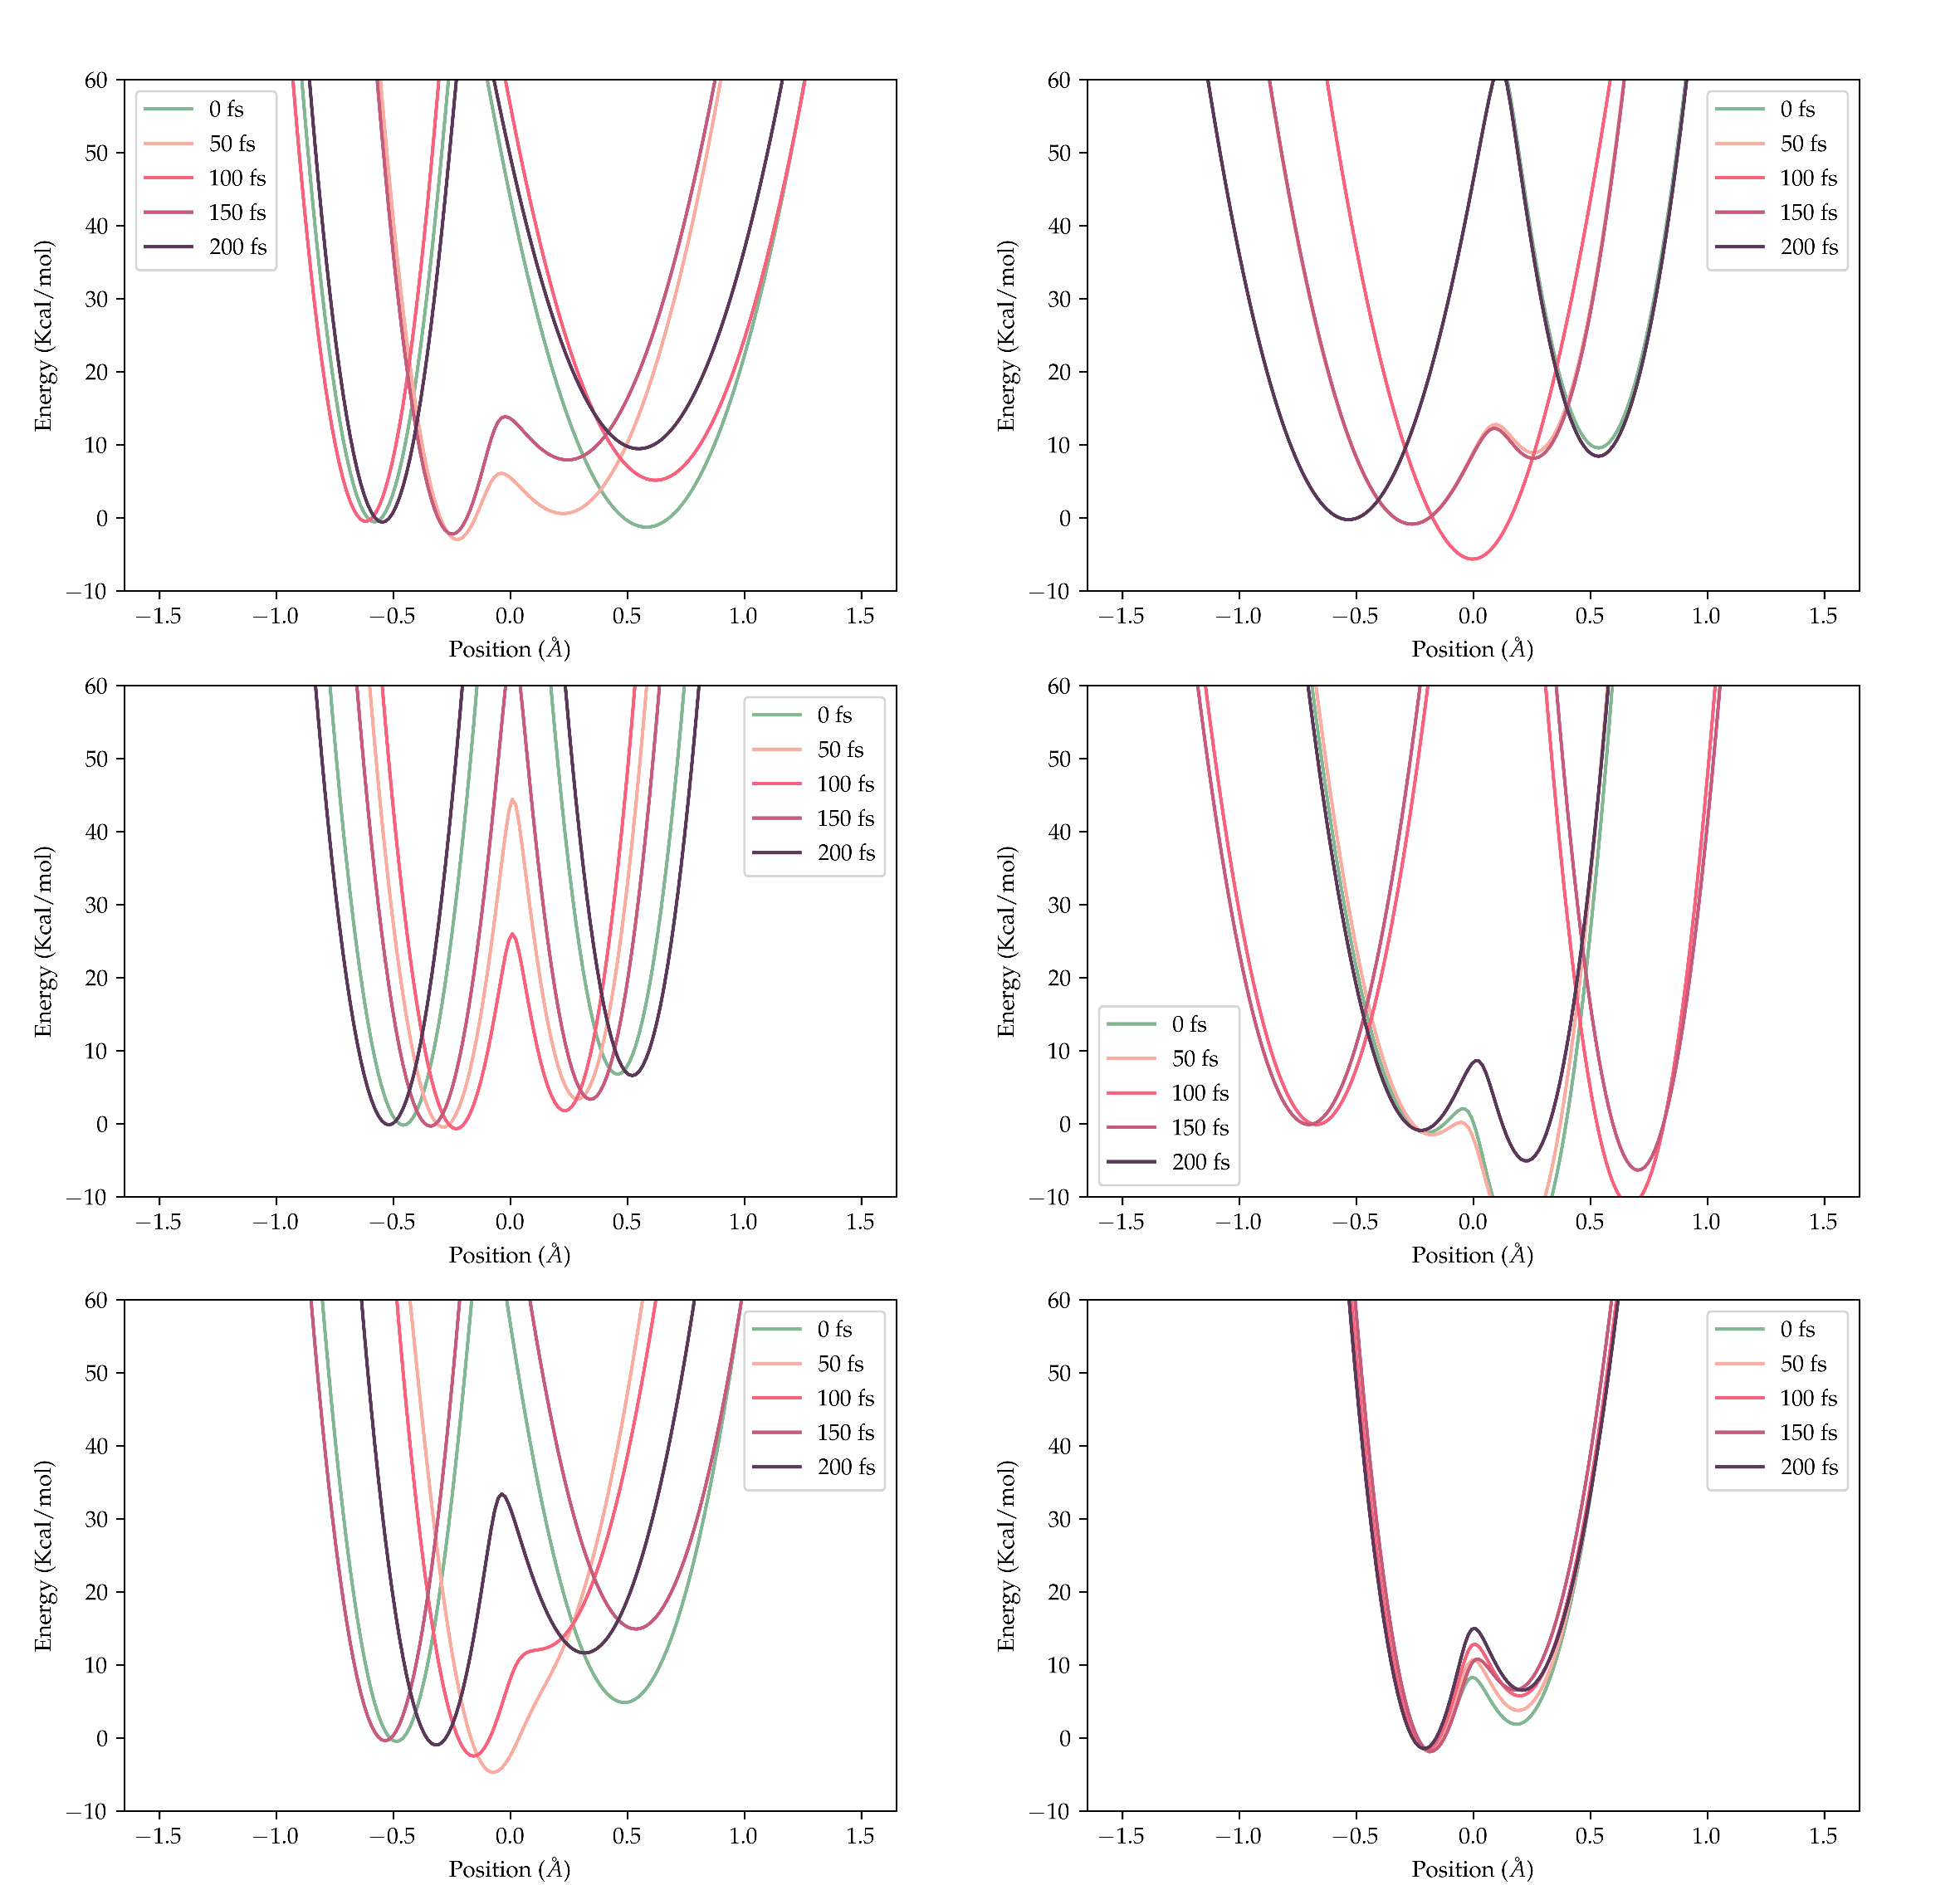
\includegraphics[width=1\textwidth]{/home/jessica/Tesis/img/tesis/ExamplesPotentialApen.png}
  \caption{Ejemplos de Potenciales utilizados $V(r,t)$}
  %\label{fig:dens_ev}
\end{figure}

\begin{figure}[!htbp]
  \centering
  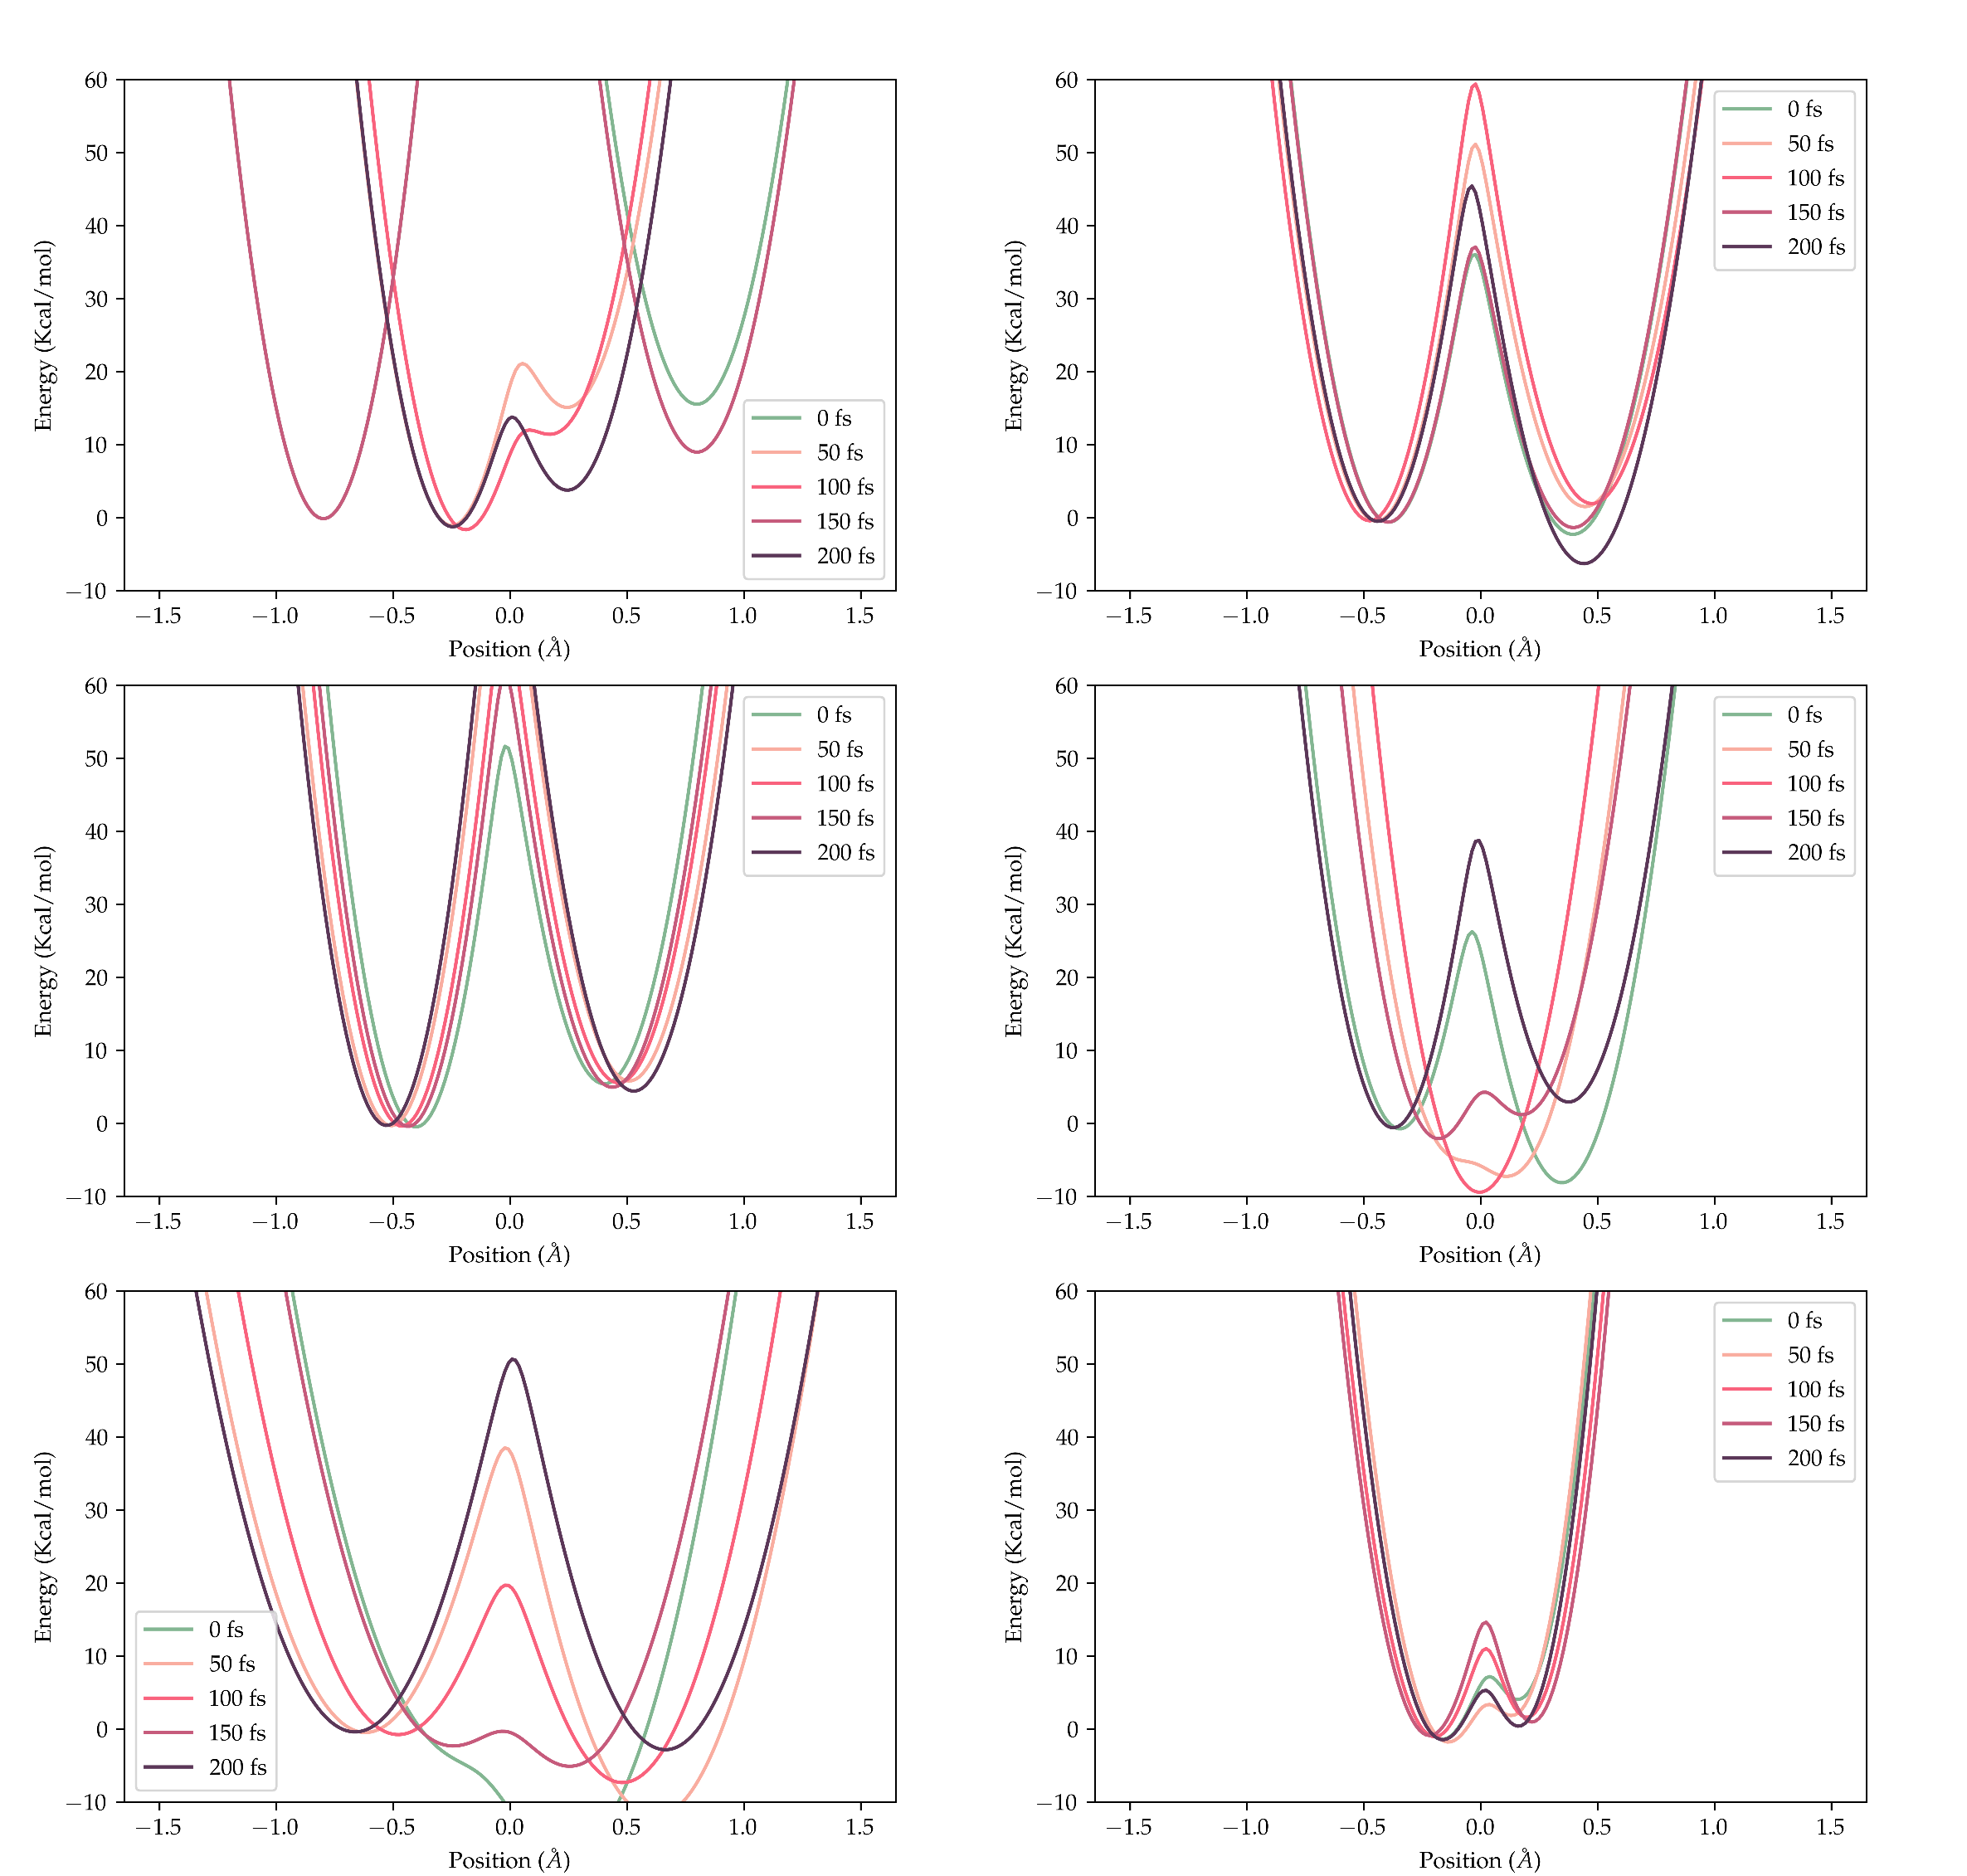
\includegraphics[width=1\textwidth]{/home/jessica/Tesis/img/tesis/ExamplesPotentialApen1.png}
  \caption{Ejemplos de Potenciales utilizados $V(r,t)$}
  %\label{fig:dens_ev}
\end{figure}




\section{Unidades Atómicas}
%\faHandshake[regular] No pelien
%------------ Tabla 1 unidades atómicas
%----------------------------------------------
\begin{table}[ht]
  \myfloatalign
  \begin{tabularx}{\textwidth}{Xll} \toprule
   \tableheadline{Unidades Atómicas} & \tableheadline{Valor SI} & \tableheadline{Nombre (símbolo)}\\ \midrule
    Masa $m_e$                  & 9.10939(-31)  & Masa del electrón     \\ \midrule
    Carga $e$                   & 1.602188(-19) & Carga del electrón \\ \midrule
    Momento angular $\hbar$     & 1.05457(-34) & Constante de Planck$/2\pi$   \\ \midrule
    Energía $(m_e e^4/\hbar^2)$  & 4.35975(-18)  & Hartree $(H)$\\ \midrule
    Longitud $(\hbar^2/m_ee^2)$  & 5.29177(-11)  & Radio de Bohr $(a_0)$\\ \midrule
    Tiempo $(\hbar^3/m_ee^4)$    & 2.41888(-17)  & Jiffy \\ \midrule
    {Momento Dipolar Eléctrico} $(\hbar^2/m_ee)$ & 8.47836(-30) & 2.541765 Debye $(D)$units  \\ \midrule
    Momento Dipolar Magnético $(e\hbar/2m_e)$  & 9.27402(-24)    & Magneton de Bohr $(\mu_B)$    \\
    \bottomrule
  \end{tabularx}
  \caption{Conversión de Unidades Atómicas a Unidades SI.}
  \label{tab:AU-SI}
\end{table}
%------------ Tabla 2 unidades atómicas Energía
%----------------------------------------------

\begin{table}[ht]
  \myfloatalign
  % \resizebox{0.5\textwidth}{!}{%
  \footnotesize
  \begin{tabularx}{\textwidth}{XXXXXX} \toprule
   Unidad      & $a.u.$ & $kcal/mol$  & $eV$        & $cm^{-1}$    & $Hz$        \\ \midrule% & $K$          \\ \midrule
    $a.u.$     & 1      & 6.27510(2) & 2.72114(1) & 2.19475(5) & 6.57968(15) \\ \midrule%& 3.15773 (5)  \\ \midrule
    $kcal/mol$ & 1.59360(-3) & 1     & 4.33641(-2)& 3.49755(2) & 1.04854(13) \\ \midrule%& 5.03217 (2)  \\ \midrule
    $eV$       & 3.67493(-2) & 2.30605(1) & 1     & 8.06554(3) & 2.41799(14) \\ \midrule%& 1.16044 (4)  \\ \midrule
    $cm^{-1}$   & 4.55634(-6) & 2.85914(-3) & 1.23984(-4) & 1   & 2.99792(10) \\ \midrule%& 1.43877      \\ \midrule
    $Hz$       & 1.51983(-16)& 9.5371(-14) & 4.13567(-15) & 3.33564(-11) & 1  \\ %\midrule& 4.79922 (-11)\\ %\midrule
   % $K$        & 3.16683 (-6) & 1.98722 (-3) & 8.61739 (-5) & 6.95039 (-1) & 2.08367 (10)& 1   \\ 
    \bottomrule
  \end{tabularx}%}
  \caption{Conversión de Energía (diversas unidades).}
  \label{tab:AU-SI}
\end{table}









%\begin{lstlisting}[float=b,language=Pascal,frame=tb,caption={A floating example (\texttt{listings} manual)},label=lst:useless]
%for i:=maxint downto 0 do
%begin
%{ do nothing }
%end;
%\end{lstlisting}

%Ei solet nemore consectetuer nam. Ad eam porro impetus, te choro omnes
%evertitur mel. Molestie conclusionemque vel at, no qui omittam
%expetenda efficiendi. Eu quo nobis offendit, verterem scriptorem ne
%vix.

